\section[
		\texttt{cognitivefactory-interactive-clustering-gui}
	]{
		Implémentation de l'application web \\ \texttt{cognitivefactory-interactive-clustering-gui}
	}
\label{annex:C.2-DESCRIPTION-IMPLEMENTATION-INTERACTIVE-CLUSTERING-GUI}

	% INTRODUCTION DE L'ANNEXE.
	La librairie \texttt{cognitivefactory-interactive-clustering-gui} \footnote{
		\url{https://pypi.org/project/cognitivefactory-interactive-clustering-gui/}
	} (\cite{schild-etal:2022:cognitivefactory-interactiveclusteringgui}) a été implémentée au cours de ce doctorat dans le but d'intégrer notre méthodologie de \texttt{Clustering Interactif} au sein d'une application web.
	Cette application dispose de plusieurs fonctionnalités telles que :
	\begin{itemize}
		\item la gestion du projet, de ses paramétrages et de ses données (cf. \textsc{Figures}~\textsc{\ref{figure:C-WEB-APPLICATION-LISTE-PROJETS}},~\textsc{\ref{figure:C-WEB-APPLICATION-ACCUEIL-PROJET}},~\textsc{\ref{figure:C-WEB-APPLICATION-PARAMETRAGE}} et~\textsc{\ref{figure:C-WEB-APPLICATION-INVENTAIRE-TEXTES}}) ;
		\item la gestion et l'annotation de contraintes, ainsi que la vérification des propriétés de transitivité (cf. \textsc{Figures}~\textsc{\ref{figure:C-WEB-APPLICATION-INVENTAIRE-CONTRAINTES}},~\textsc{\ref{figure:C-WEB-APPLICATION-ANNOTATION}} et~\textsc{\ref{figure:C-WEB-APPLICATION-CONFLIT}}) ;
		\item la gestion des étapes d'une itération et de l'exécution asynchrone des divers algorithmes (cf. \textsc{Figures}~\textsc{\ref{figure:C-WEB-APPLICATION-ACCUEIL-PROJET}} et~\textsc{\ref{figure:C-WEB-APPLICATION-DIAGRAMME-ETATS}}) ;
		\item quelques scripts d'analyses.
	\end{itemize}
	
	Nous présentons succinctement cette application ci-dessous à l'aide de captures d'écrans.

	
	% Information : comme y accéder.
	\begin{leftBarInformation}
		La documentation technique de cette librairie est accessible au lien suivant : \url{https://cognitivefactory.github.io/interactive-clustering-gui/}.
	\end{leftBarInformation}
	
	% Information : projet ingénieur TPS
	\setcounter{localCounterOfFootnoteValue}{\value{footnote}}
	\begin{leftBarAuthorOpinion}
		L'étude d'une interface graphique et de ses fonctionnalités a été l'objet d'un premier projet étudiant avec l'école d'ingénieur Télécom Physique Strasbourg (au cours de l'année 2021).
		Lors de nos échanges, une idée consistait à s'inspirer des fonctionnalités de l'application \texttt{TINDER} \footnotemark pour \textit{swipe left} (respectivement \textit{swipe right}) l'annotation d'une contrainte \texttt{MUST-LINK} (respectivement d'une contrainte \texttt{CANNOT-LINK}).
		Bien qu'aucune version mobile de cette application n'a été développée, une telle fonctionnalité pourrait être envisagée afin d'améliorer le confort de l'utilisateur.
		Nous pouvons toutefois noter qu'un reliquat de cette discussion à mener au choix du logo de l'application, proche du logo de celui de l'application \texttt{TINDER}, ainsi qu'au design de la page d'annotation (cf. \textsc{Figure~\ref{figure:C-WEB-APPLICATION-ANNOTATION}}).
	\end{leftBarAuthorOpinion}
		% Rattraper les footnote.
			\stepcounter{localCounterOfFootnoteValue}
			\footnotetext[\value{localCounterOfFootnoteValue}]{
				\url{https://tinder.com/fr}
			}
	
	% Note de l'auteur : en cours de maintenance.
	\begin{leftBarAuthorOpinion}
		Suite aux diverses études menées au cours de ce doctorat, certaines pages sont en cours de développement, notamment :
		\begin{itemize}
			\item les pages d'analyses dont le but d'intégrer les conclusions du \textsc{Chapitre~\ref{chapter:4-ETUDES}} ;
			\item les pages de documentation pour intégrer les discussions du \textsc{Chapitre~\ref{chapter:5-GUIDE}}.
		\end{itemize}
	\end{leftBarAuthorOpinion}
	
	
	%%%
	%%% Subsection C.2.1: Accueil et Gestion de projets.
	%%%
	\newpage
	\subsection{Accueil et Gestion de projets}
	\label{annex:C.2.1-DESCRIPTION-IMPLEMENTATION-INTERACTIVE-CLUSTERING-GUI-ACCUEIL}
	
		%%% Page d'accueil de l'application
		%\newpage
		\paragraph{Page d'accueil de l'application (\textsc{Figure~\ref{figure:C-WEB-APPLICATION-ACCUEIL}}) :}
			
			% Capture d'écran: Page d'accueil de l'application.
			\begin{figure}[H]
				\centering
				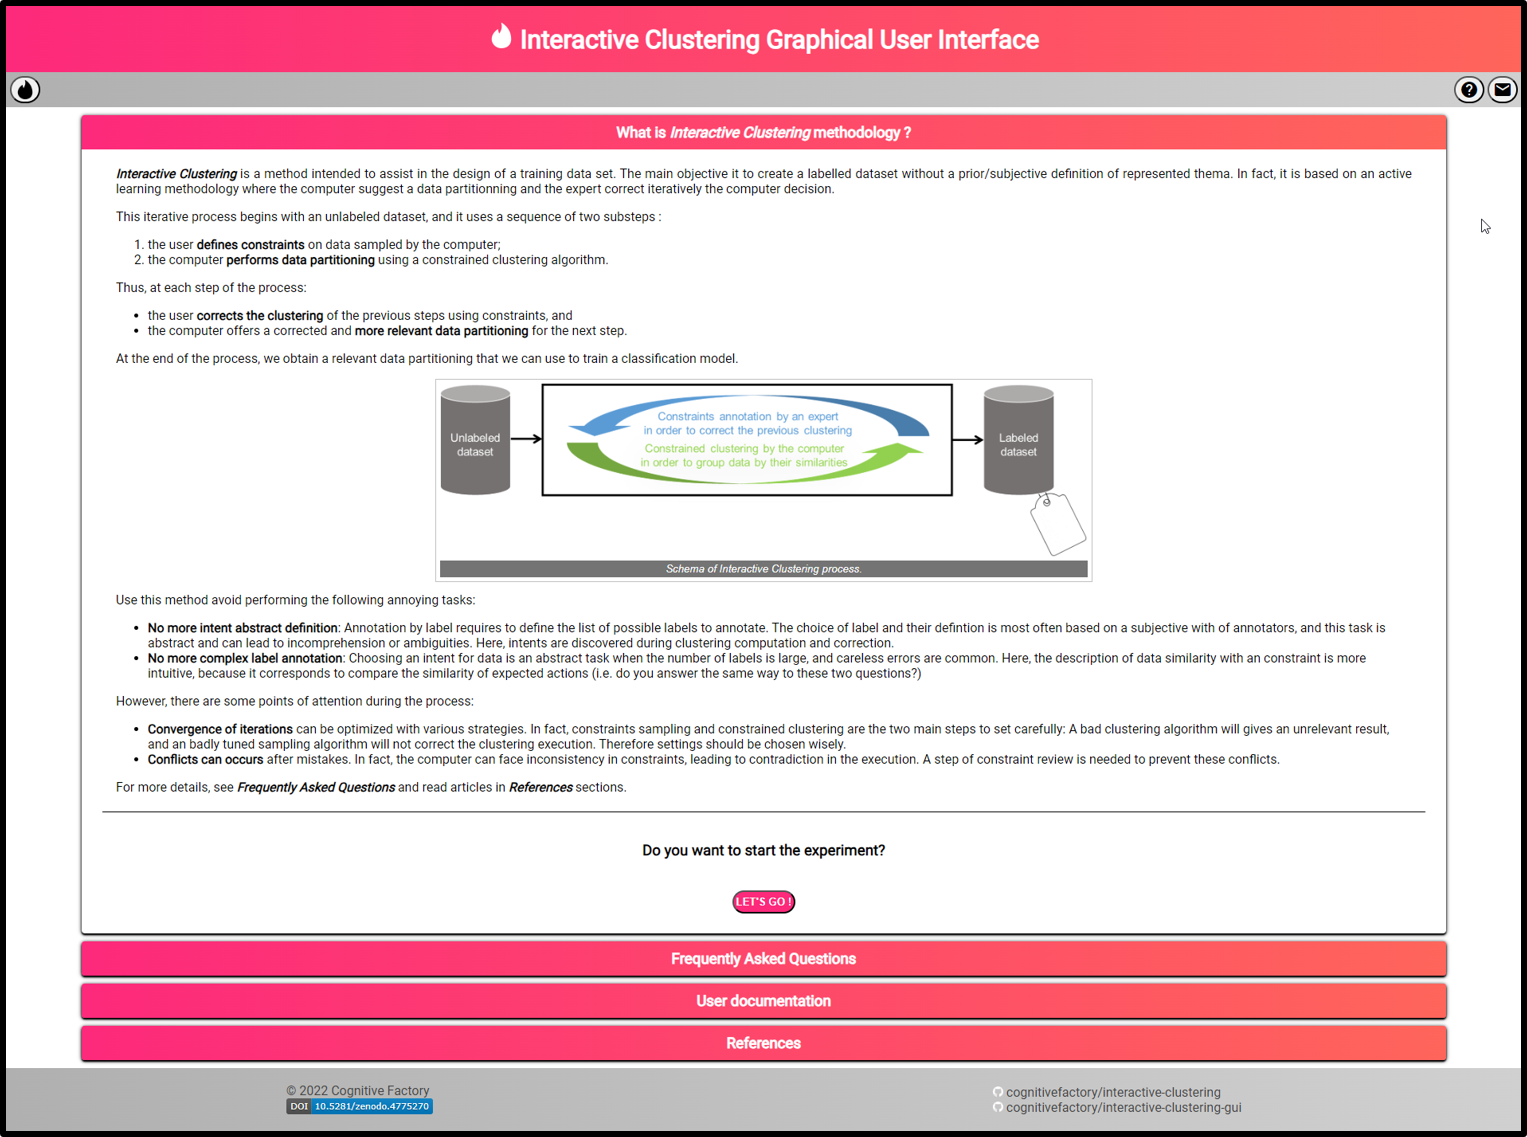
\includegraphics[width=0.95\textwidth]{figures/interactive-clustering-application-accueil-application}
				\caption{
					Capture d'écran de l'application web implémentant notre méthodologie de \texttt{Clustering Interactif} : \textbf{page d'accueil de l'application}.
				}
				\label{figure:C-WEB-APPLICATION-ACCUEIL}
			\end{figure}
			
			% Description générale.
			C'est la page de bienvenu de l'application.
			Nous y trouvons une description rapide de la méthode ainsi qu'une liste des questions fréquentes à son sujet.
			A terme, la documentation de la méthodologie d'annotation y sera intégrée (cf. discussions du \textsc{Chapitre~\ref{chapter:5-GUIDE}}).
			
			% Boutons accessibles.
			Concernant les boutons accessibles :
			\begin{itemize}
				\item Le bouton d'accueil en haut à gauche redirigera toujours sur cette page ;
				\item Le bouton de contact en haut à droite permet de contacter l'équipe de recherche ;
				\item Le bouton \textguillemets{\texttt{LET'S GO}} permet d'accéder à la page de listant les projets d'annotation (cf. \textsc{Figure~\ref{figure:C-WEB-APPLICATION-LISTE-PROJETS}}).
			\end{itemize}
			
			% Information : comme y accéder.
			\begin{leftBarInformation}
				Dans toutes les pages suivantes, il est à noter que :
				\begin{itemize}
					\item Tous les boutons peuvent être survolés pour afficher une courte description de leur action ou de leur état, ainsi que les raccourcis clavier qui permettent de les activer ;
					\item Si besoin, tous les encadrés sont repliables pour gagner en visibilité.
				\end{itemize}
			\end{leftBarInformation}
		
		
		%%% Page de gestion des projets
		%\newpage
		\paragraph{Page de gestion des projets (\textsc{Figure~\ref{figure:C-WEB-APPLICATION-LISTE-PROJETS}}) :}
			
			% Capture d'écran: liste des projets.
			\begin{figure}[H]
				\centering
				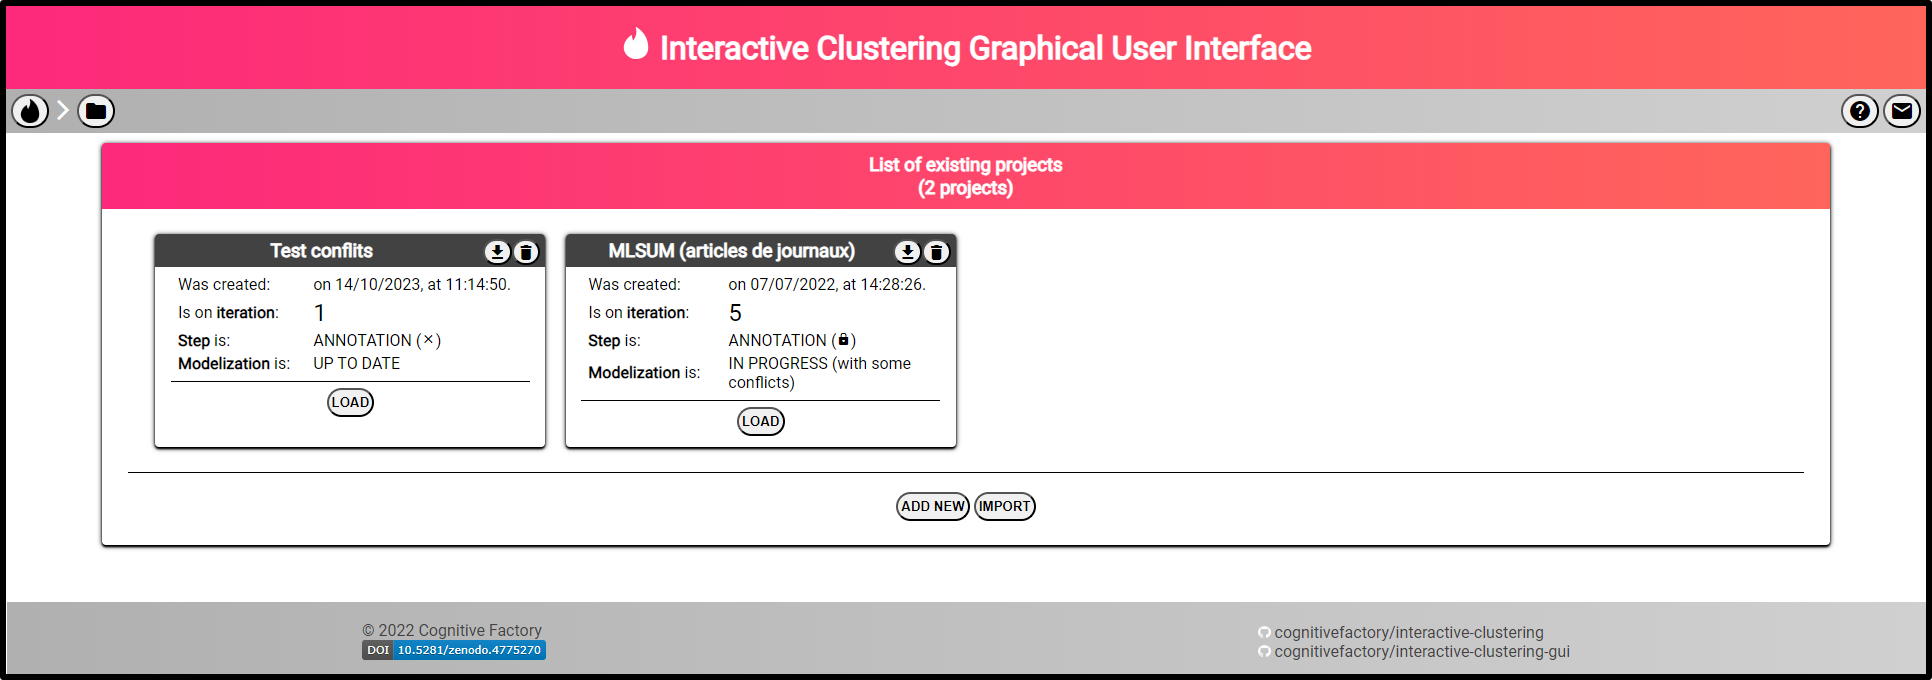
\includegraphics[width=0.95\textwidth]{figures/interactive-clustering-application-liste-projets}
				\caption{
					Capture d'écran de l'application web implémentant notre méthodologie de \texttt{Clustering Interactif} : \textbf{page de gestion des projets}.
				}
				\label{figure:C-WEB-APPLICATION-LISTE-PROJETS}
			\end{figure}
			
			% Description générale.
			Cette page liste les projets existants sous la forme de tuiles contenant les informations importantes : nom, date de création, nombre d'itérations de la méthode, et l'état du projet (cf. \textsc{Figure~\ref{figure:C-WEB-APPLICATION-DIAGRAMME-ETATS}}).
			
			% Boutons accessibles.
			Concernant les boutons d'action de cette page :
			\begin{itemize}
				\item Les boutons d'accueil en haut à gauche permettent de naviguer entre cette page et la page d'accueil de l'application (cf. \textsc{Figure~\ref{figure:C-WEB-APPLICATION-ACCUEIL}}) ;
				\item Il est possible de télécharger un projet au format \texttt{.zip} ou de le supprimer grâce aux boutons \textguillemets{\faDownload} et \textguillemets{\faTrash} en haut à droite de chaque tuile ;
				\item Pour créer un projet, le bouton \textguillemets{\texttt{ADD NEW}} ouvre un formulaire demandant le nom du projet et la liste des textes à annoter (fichier au format \texttt{.csv} avec séparateur '\texttt{;}') ;
				\item Il est aussi possible d'importer un projet contenu dans une archive \texttt{.zip} grâce au bouton \textguillemets{\texttt{IMPORT}} ;
				\item Enfin, le bouton \textguillemets{\texttt{LOAD}} mène à la page d'accueil du projet sélectionné (cf. \textsc{Figure~\ref{figure:C-WEB-APPLICATION-ACCUEIL-PROJET}}).
			\end{itemize}
	
	
	%%%
	%%% Subsection C.2.2: Projet, Diagramme d'états et Paramétrages.
	%%%
	\newpage
	\subsection{Projet, Diagramme d'états et Paramétrages}
	\label{annex:C.2.2-DESCRIPTION-IMPLEMENTATION-INTERACTIVE-CLUSTERING-GUI-PROJET}
	
		%%% Page d'accueil du projet en cours
		%\newpage
		\paragraph{Page d'accueil du projet en cours (\textsc{Figure~\ref{figure:C-WEB-APPLICATION-ACCUEIL-PROJET}}) :}
			
			% Capture d'écran: accueil projet.
			\begin{figure}[H]
				\centering
				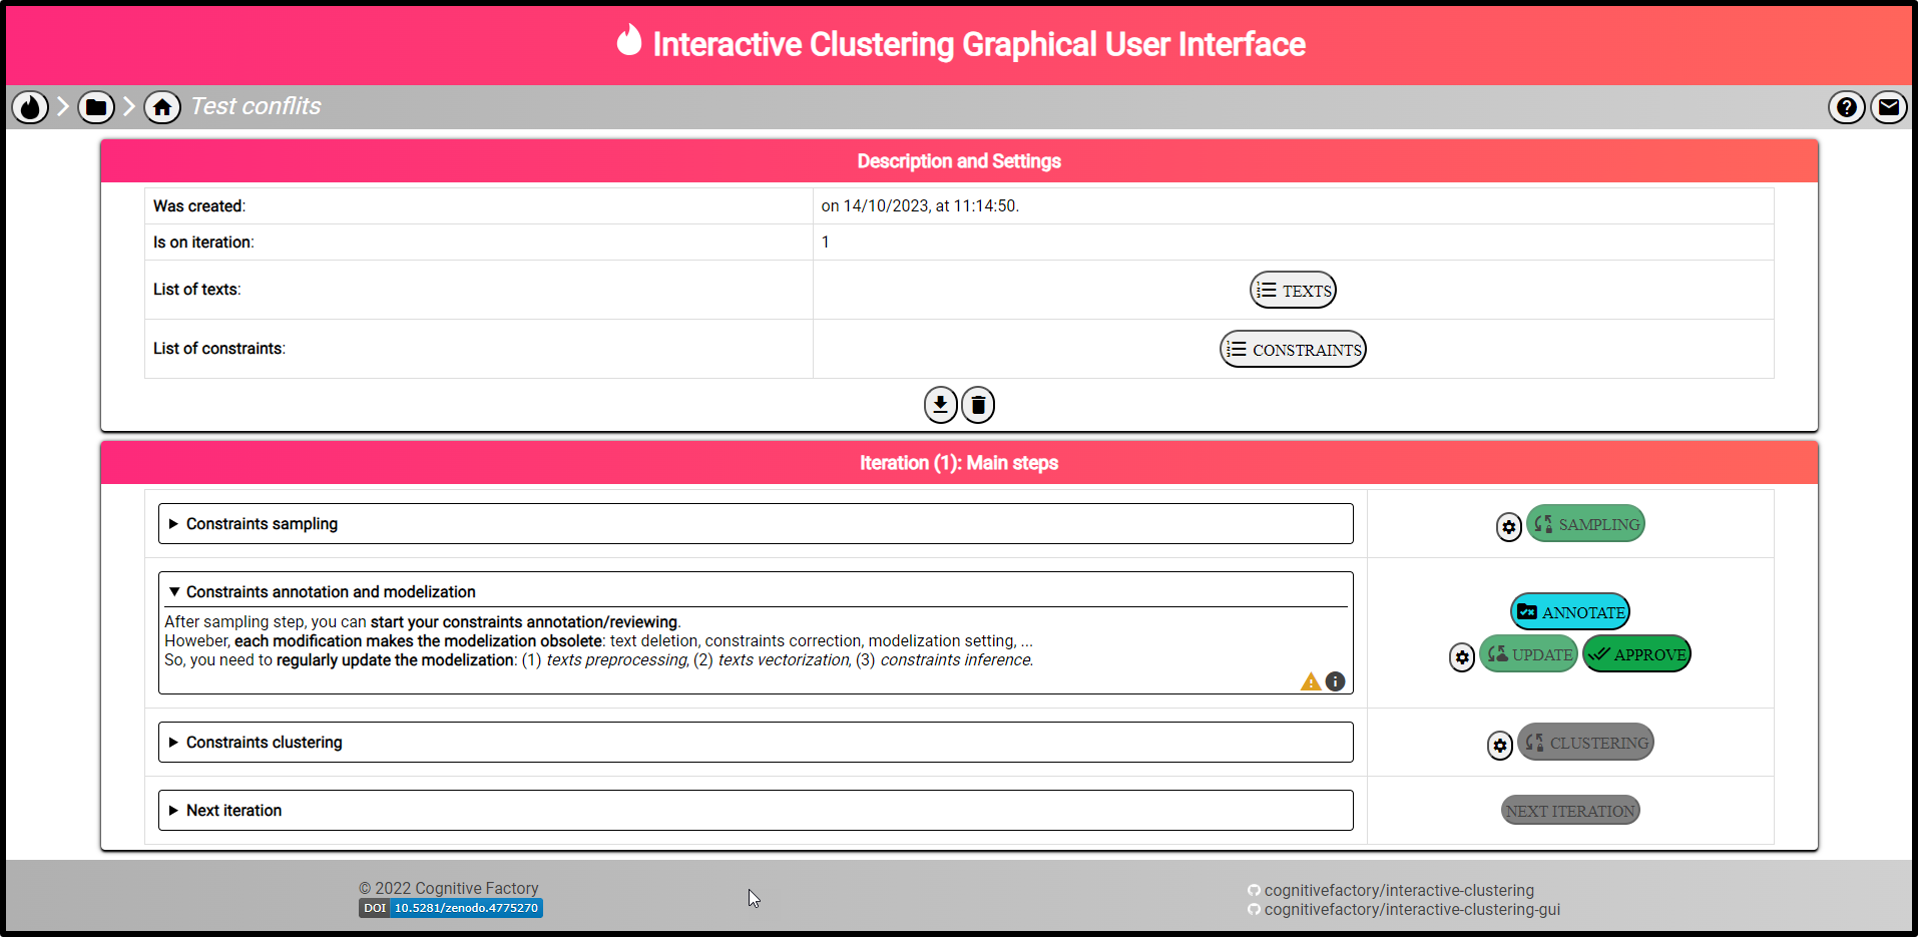
\includegraphics[width=0.95\textwidth]{figures/interactive-clustering-application-accueil-projet}
				\caption{
					Capture d'écran de l'application web implémentant notre méthodologie de \texttt{Clustering Interactif} : \textbf{page d'accueil du projet en cours}.
				}
				\label{figure:C-WEB-APPLICATION-ACCUEIL-PROJET}
			\end{figure}
			
			% Description générale.
			C'est la page principale de l'application.
			Elle contient en partie supérieure les informations du projet d'annotation en cours (\textit{date de création, numéro d'itération, gestion des textes et des contraintes}), et en partie inférieure les étapes d'une itération de \texttt{Clustering Interactif} (\textit{descriptions, boutons d'actions et de paramétrages}).
			
			% Boutons accessibles: gestion de projet.
			Concernant la gestion du projet (partie supérieure) :
			\begin{itemize}
				\item Les boutons d'accueil en haut à gauche permettent de naviguer entre cette page, la page de gestion des projets (cf. \textsc{Figure~\ref{figure:C-WEB-APPLICATION-LISTE-PROJETS}} et la page d'accueil de l'application (cf. \textsc{Figure~\ref{figure:C-WEB-APPLICATION-ACCUEIL}}) ;
				\item Au centre, il est possible de télécharger le projet au format \texttt{.zip} ou de le supprimer grâce aux boutons \textguillemets{\faDownload} et \textguillemets{\faTrash} ;
				\item Le bouton \textguillemets{\texttt{TEXTS}} mène vers la page d'inventaire et de gestion des textes du projet (cf. \textsc{Figure~\ref{figure:C-WEB-APPLICATION-INVENTAIRE-TEXTES}}) ;
				\item Le bouton \textguillemets{\texttt{CONSTRAINTS}} mène vers la page d'inventaire et de gestion des contraintes annotées ou en cours d'annotation (cf. \textsc{Figure~\ref{figure:C-WEB-APPLICATION-INVENTAIRE-CONTRAINTES}}).
			\end{itemize}
			
			% Boutons accessibles: gestion d'une itération.
			Concernant la gestion d'une itération de \texttt{Clustering Interactif} (partie inférieure), les différentes étapes sont représentées de bas en haut à l'aide d'éléments descriptifs repliables et de boutons d'actions.
			Nous retrouvons quatre étapes :
			\begin{enumerate}
				\item l'échantillonnage de contraintes, exécuté en tâche de fond grâce au bouton \textguillemets{\texttt{SAMPLING}}, et dont les paramètres sont accessibles via le bouton \textguillemets{\faCog} ;
				\item l'annotation de contraintes, avec le bouton \textguillemets{\texttt{ANNOTATE}} qui redirige vers la prochaine contrainte à annoter.
				Cette étape contient aussi une gestion de la modélisation, c'est-à-dire une vérification des prétraitements et de la vectorisation des textes, ainsi qu'une vérification de la cohérence des contraintes par l'absence de conflits d'annotation : le bouton \textguillemets{\texttt{UPDATE}} permet de recalculer cette modélisation en tâche de fond et le bouton \textguillemets{\texttt{APPROVE}} permet de la fixer jusqu'à la fin de l'itération en cours ;
				\item l'\textit{clustering} sous contraintes, exécuté en tâche de fond grâce au bouton \textguillemets{\texttt{CLUSTERING}}, et dont les paramètres sont accessibles via le bouton \textguillemets{\faCog} ;
				\item la confirmation du passage à la nouvelle itération, exécutée grâce au bouton \textguillemets{\texttt{NEXT ITERATION}}.
			\end{enumerate}
			
			% Notes:
			Il est à noter que :
			\begin{itemize}
				\item Les éléments de gauche sont repliables : au chargement de la page, seul l'élément de l'étape en cours est déplié ;
				\item La gestion de l'itération se fait à l'aide d'un diagramme d'état (cf. \textsc{Figure~\ref{figure:C-WEB-APPLICATION-DIAGRAMME-ETATS}}) : celui-ci se manifeste par un code couleur et l'activation/désactivation des boutons.
			\end{itemize}
		
		
		%%% Diagramme d'états de l'application et gestion des exécutions asynchrones
		%\newpage
		\paragraph{Diagramme d'états de l'application et gestion des exécutions asynchrones (\textsc{Figure~\ref{figure:C-WEB-APPLICATION-DIAGRAMME-ETATS}}) :}
			
			% Capture d'écran: accueil projet.
			\begin{figure}[H]
				\centering
				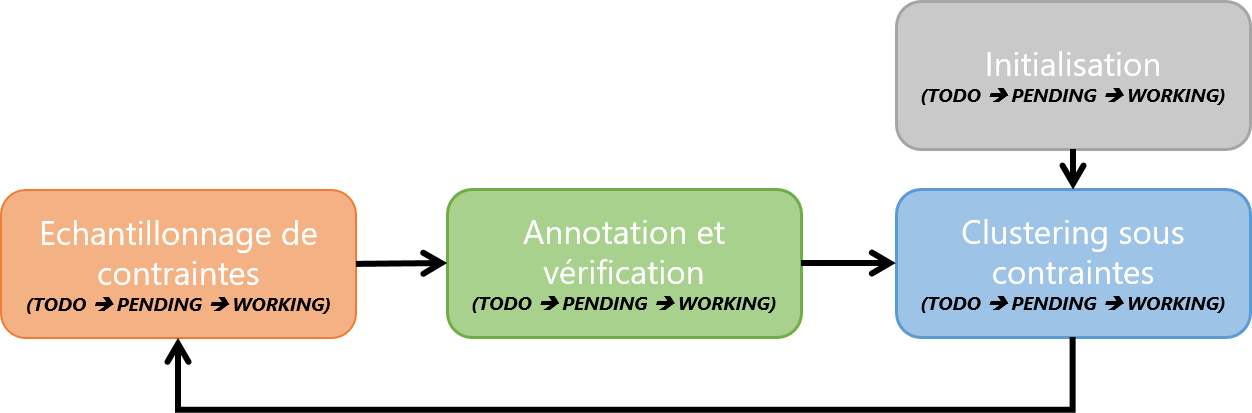
\includegraphics[width=0.95\textwidth]{figures/interactive-clustering-application-diagramme-etats}
				\caption{
					\textbf{Diagramme d'états} simplifié de l'application web implémentant notre méthodologie de \texttt{Clustering Interactif}.
				}
				\label{figure:C-WEB-APPLICATION-DIAGRAMME-ETATS}
			\end{figure}
			
			% Description générale.
			Comme décrit en \textsc{Section~\ref{section:3.2-DESCRIPTION-THEORIQUE}} et dans la \textsc{Figure~\ref{figure:3.2.1-DESCRIPTION-THEORIQUE-GENERALE}}, une itération de \textit{Clustering Interactif} contient trois étapes majeures : \textbf{(1)} l'échantillonnage de contraintes, \textbf{(2)} l'annotation de contraintes, et \textbf{(3)} le \textit{clustering} sous contraintes.
			Ces étapes sont représentées par le diagramme d'état en \textsc{Figure~\ref{figure:C-WEB-APPLICATION-DIAGRAMME-ETATS}} : ce dernier définit l'activation ou la désactivation des boutons d'action de l'application (cf. \textsc{Figure~\ref{figure:C-WEB-APPLICATION-ACCUEIL-PROJET}}).
			
			% Gestion de couleur.
			Afin de représenter l'état en cours et les actions possibles de manière pragmatique dans l'interface, un code couleur implicite est utilisé en plus de l'activation/désactivation des boutons :
			\begin{itemize}
				\item objet \textguillemets{\textcolor{colorApplicationNOTAVAILABLE}{\textbf{grisé}}} et généralement désactivé : action inaccessible pour le moment ;
				\item objet en \textguillemets{\textcolor{colorApplicationAVAILABLE}{\textbf{vert}}} et activé : prochaine action à réaliser ;
				\item objet en \textguillemets{\textcolor{colorApplicationWORKING}{\textbf{cyan}}} : action en cours de traitement ;
				\item objet en \textguillemets{\textcolor{colorApplicationERROR}{\textbf{rouge}}} et activé : action en erreur ou à recommencer ;
				\item objet en \textguillemets{\textcolor{colorApplicationDONE}{\textbf{vert grisé}}} et généralement désactivé : action réalisée avec succès.
			\end{itemize}
			
			% Gestion des actions asynchrones.
			D'autre part, comme certains algorithmes peuvent être lents, ces derniers sont exécutés en tâche de fond.
			La gestion d'état est alors affinée en quatre sous-états :
			\begin{itemize}
				\item \textguillemets{\textcolor{colorApplicationAVAILABLE}{\textbf{\texttt{TODO}}}} : l'action est à faire, la machine attend l'ordre de l'utilisateur ;
				\item \textguillemets{\textcolor{colorApplicationWORKING}{\textbf{\texttt{PENDING}}}} : l'action a été ordonnée par l'utilisateur, mais elle n'a pas encore été prise en charge par la machine ;
				\item \textguillemets{\textcolor{colorApplicationWORKING}{\textbf{\texttt{WORKING}}}} : l'action est en cours d'exécution en tâche de fond.
				Une barre d'avancement apparaît pour maintenir l'utilisateur informé de l'évolution de cet état ;
				\item \textit{Note} : l'état \textguillemets{\textcolor{colorApplicationDONE}{\textbf{\texttt{DONE}}}} (action faite) n'existe pas réellement, elle est représentée par le fait que la prochaine étape ait un état \textguillemets{\texttt{TODO}}.
			\end{itemize}
			
			% Warning: Architecture asynchrone en production.
			\begin{leftBarWarning}
				Pour une simplicité d'usage et afin d'offrir une démonstration rapide de notre méthodologie, nous avons décidé d'exécuter simplement les algorithmes en tâche de fond.
				Toutefois, pour favoriser les performances de l'application ainsi que sa sûreté pour une utilisation en production, nous vous conseillons de ré-implémenter cette gestion des exécutions en privilégiant une architecture asynchrone utilisant des \textit{workers} dédiés.
			\end{leftBarWarning}
		
		
		%%% Page de gestion des paramètres
		%\newpage
		\paragraph{Page de gestion des paramètres (\textsc{Figure~\ref{figure:C-WEB-APPLICATION-PARAMETRAGE}}) :}
		
			% Capture d'écran: gestion des paramètrages.
			\begin{figure}[H]
				\centering
				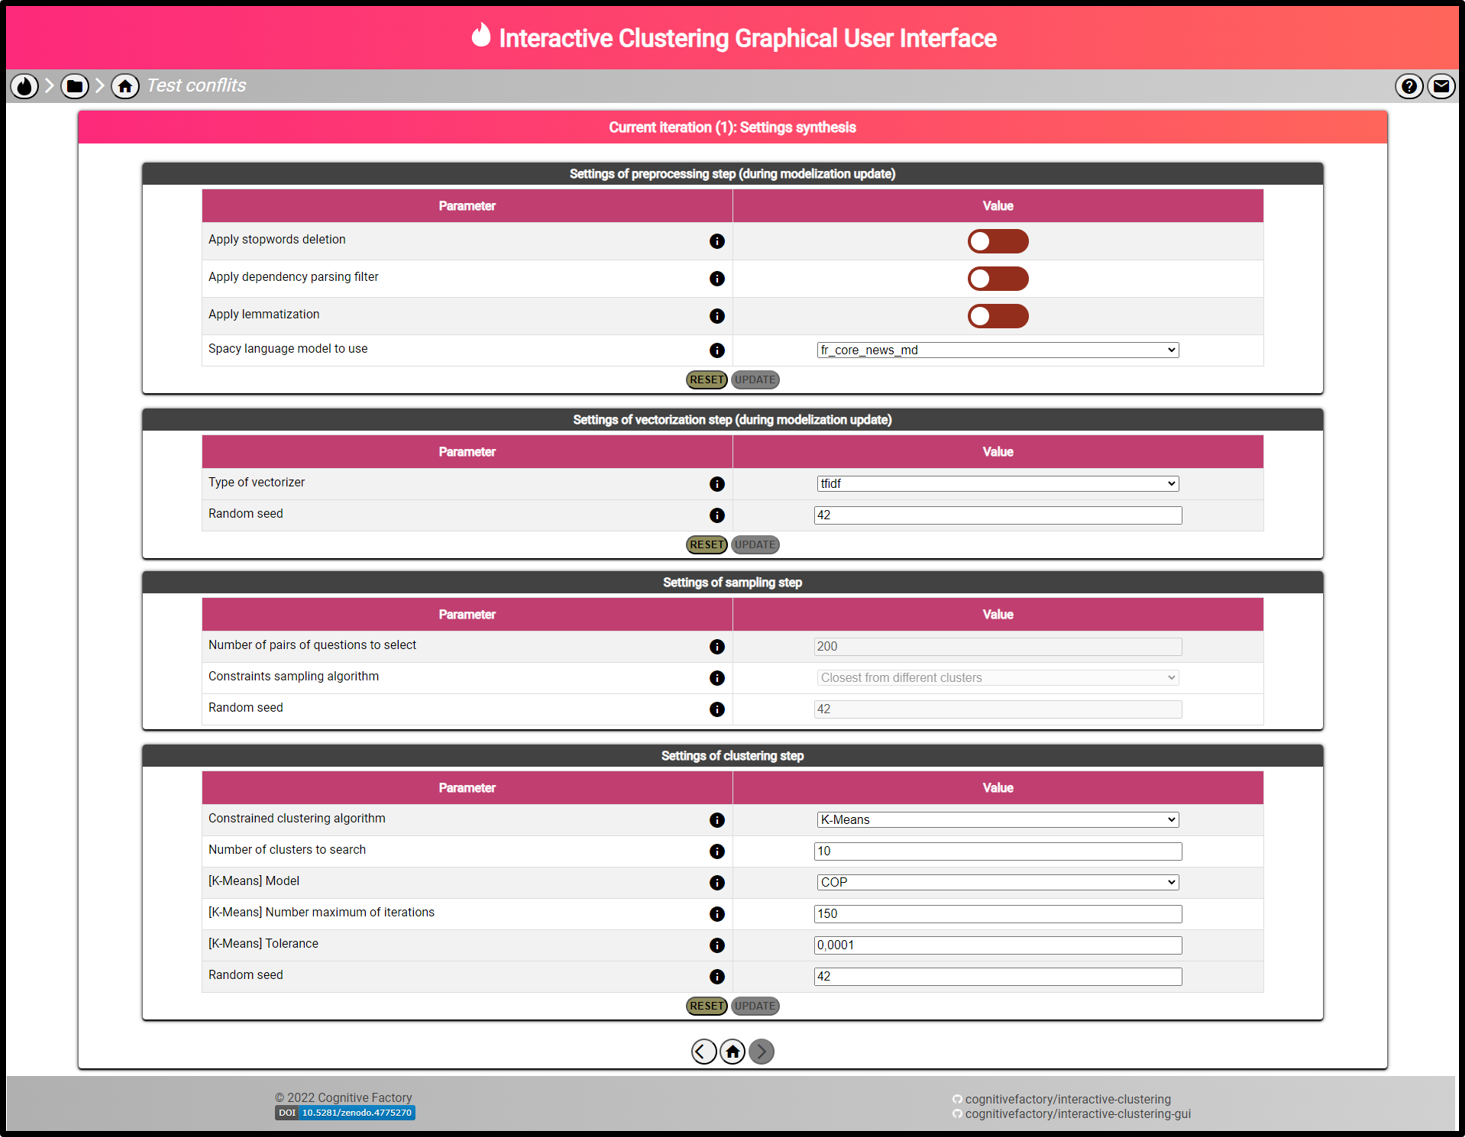
\includegraphics[width=0.95\textwidth]{figures/interactive-clustering-application-parametres}
				\caption{
					Capture d'écran de l'application web implémentant notre méthodologie de \texttt{Clustering Interactif} : \textbf{page de gestion des paramètres}.
				}
				\label{figure:C-WEB-APPLICATION-PARAMETRAGE}
			\end{figure}
			
			% Description générale.
			Accessible depuis les différents boutons \textguillemets{\faCog}, cette page liste les divers paramètres des algorithmes pour chaque itération.
			\begin{itemize}
				\item Chaque tuile représente une tâche (prétraitements, vectorisation, échantillonnage et \textit{clustering}) : divers algorithmes et hyperparamètres son disponibles ;
				\item Les boutons \textguillemets{\texttt{UPDATE}} permettent de valider les changements, les boutons \textguillemets{\texttt{RESET}} rétablissent les paramètres par défaut ;
				\item Ces différents formulaires sont modifiables tant que l'étape n'est pas en cours d'exécution, sinon ils sont juste consultables ;
				\item En bas de page, il est possible de changer d'itération pour consulter les paramètres des itérations précédentes (boutons \textguillemets{\faAngleLeft} et \textguillemets{\faAngleRight}), et de revenir vers la page d'accueil du projet (bouton \textguillemets{\faHome}, cf. \textsc{Figure~\ref{figure:C-WEB-APPLICATION-ACCUEIL-PROJET}}).
			\end{itemize}
	
	
	%%%
	%%% Subsection C.2.3: Textes et Contraintes.
	%%%
	\newpage
	\subsection{Textes et Contraintes}
	\label{annex:C.2.3-DESCRIPTION-IMPLEMENTATION-INTERACTIVE-CLUSTERING-GUI-DONNEES}
	
		%%% Page d'inventaire des textes
		%\newpage
		\paragraph{Page d'inventaire des textes (\textsc{Figure~\ref{figure:C-WEB-APPLICATION-INVENTAIRE-TEXTES}}) :}
		
			% Capture d'écran: inventaire des textes.
			\begin{figure}[H]
				\centering
				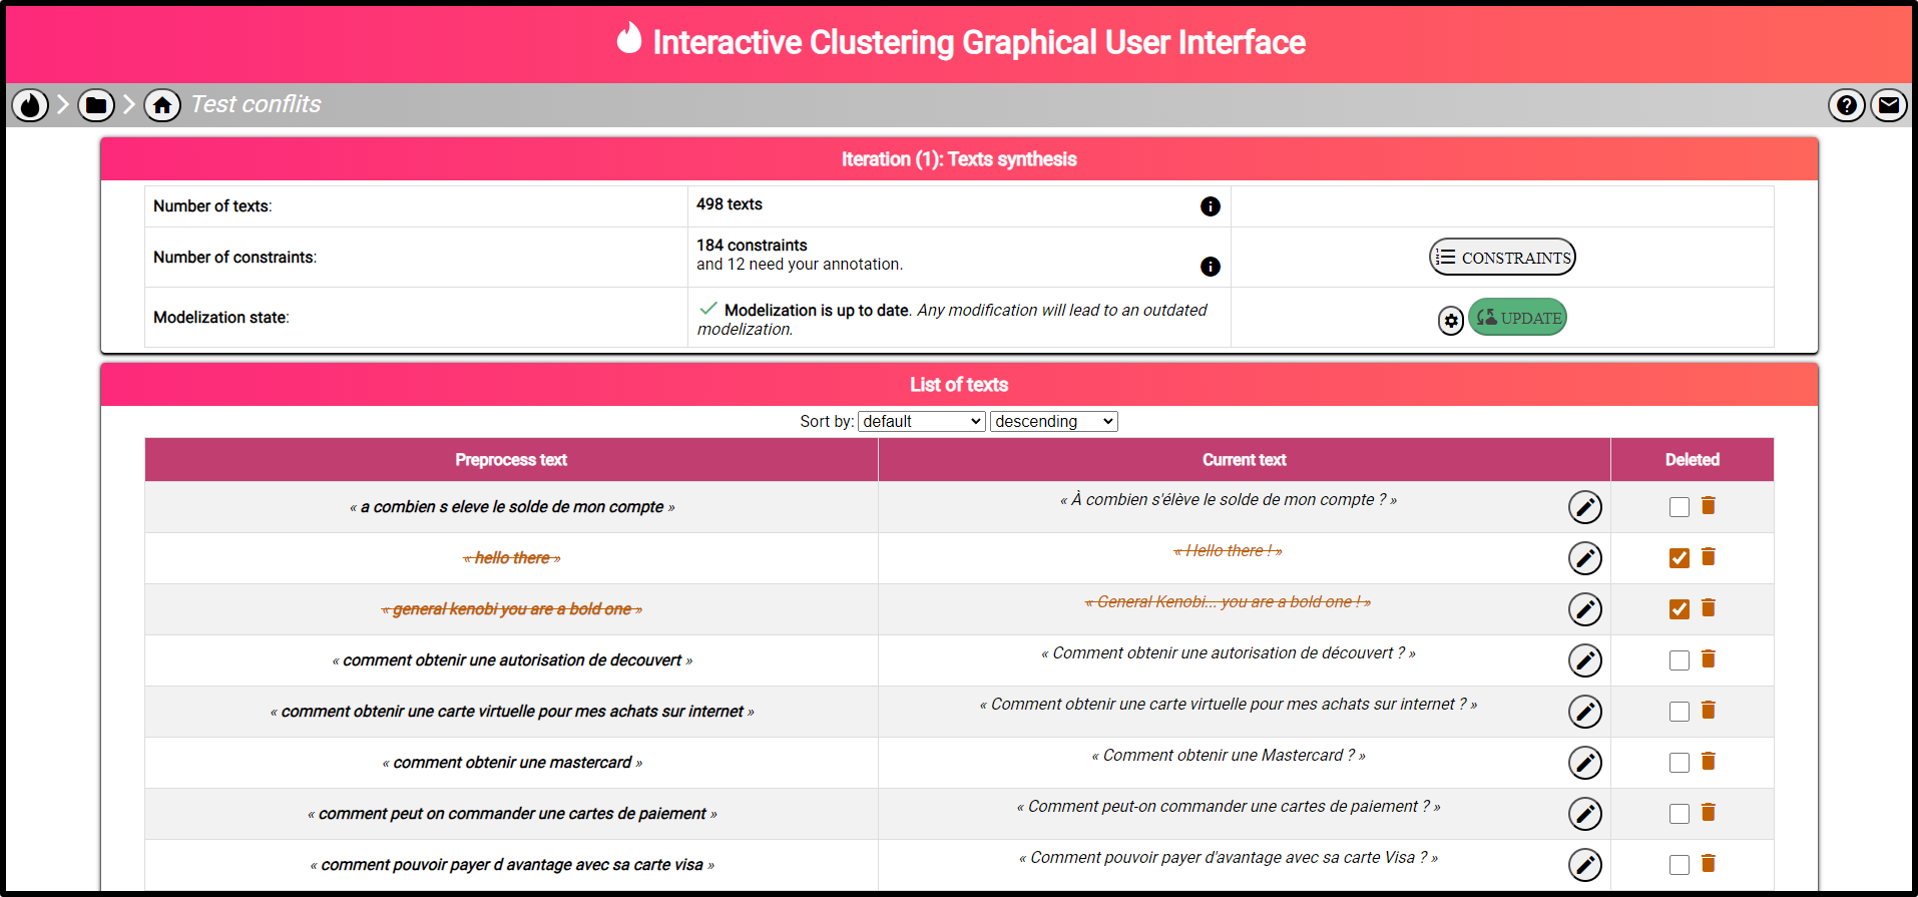
\includegraphics[width=0.95\textwidth]{figures/interactive-clustering-application-textes}
				\caption{
					Capture d'écran de l'application web implémentant notre méthodologie de \texttt{Clustering Interactif} : \textbf{page d'inventaire des textes}.
				}
				\label{figure:C-WEB-APPLICATION-INVENTAIRE-TEXTES}
			\end{figure}
			
			% Description générale.
			Cette page permet de lister les textes du projet à annoter.
			La page est divisée en deux : la partie supérieure donne des informations générales (\textit{nombre de textes, nombre de contraintes à annoter, rappel de la modélisation en cours}), et la partie inférieure liste les textes dans un tableau.
			
			% Boutons accessibles: gestion des textes.
			Concernant les informations générales (partie supérieure) :
			\begin{itemize}
				\item Le bouton \textguillemets{\texttt{UPDATE}} permet de mettre à jour la modélisation si des contraintes ont été ajoutées, des paramètres de prétraitements ou de vectorisation ont été mis à jour, ou si des textes ont été modifiés : cette action est exécutée en tâche de fond.
				La couleur de se bouton est définie par le diagramme d'état (cf. \textsc{Figure~\ref{figure:C-WEB-APPLICATION-DIAGRAMME-ETATS}}) ;
				\item Le bouton \textguillemets{\texttt{CONSTRAINTS}} mène vers la page d'inventaire et de gestion des contraintes annotées ou en cours d'annotation (cf. \textsc{Figure~\ref{figure:C-WEB-APPLICATION-INVENTAIRE-CONTRAINTES}}).
			\end{itemize}
			
			% Boutons accessibles: liste des textes.
			Concernant le tableau listant les textes (partie inférieure) :
			\begin{itemize}
				\item Le texte brut et sa version prétraitée sont affichés ;
				\item Grâce au bouton \textguillemets{\faPen}, il est possible de corriger un texte s'il contient une faute de frappe ;
				\item Grâce au bouton \textguillemets{\textcolor{colorApplicationDELETE}{\faTrash}}, il est possible de supprimer (\textit{ne plus prendre en compte}) un texte s'il n'est pas pertinent pour le projet : celui-ci est alors rayé en \textcolor{colorApplicationDELETE}{orange} ;
				\item En haut du tableau, il est possible de trier les textes suivant différents critères (\textit{ordre alphabétique, supprimé ou non, ...}) ;
				\item \textbf{Attention} : Toute action de modification (renommage, suppression) nécessite de mettre à jour la modélisation par la suite.
				De plus, ces actions sont désactivées si le projet n'est pas à l'étape d'annotation (cf. diagramme d'états en \textsc{Figure~\ref{figure:C-WEB-APPLICATION-DIAGRAMME-ETATS}}) ;
			\end{itemize}
		
		
		%%% Page d'inventaire des contraintes
		%\newpage
		\paragraph{Page d'inventaire des contraintes (\textsc{Figure~\ref{figure:C-WEB-APPLICATION-INVENTAIRE-CONTRAINTES}}) :}
		
			% Capture d'écran: inventaire des contraintes.
			\begin{figure}[H]
				\centering
				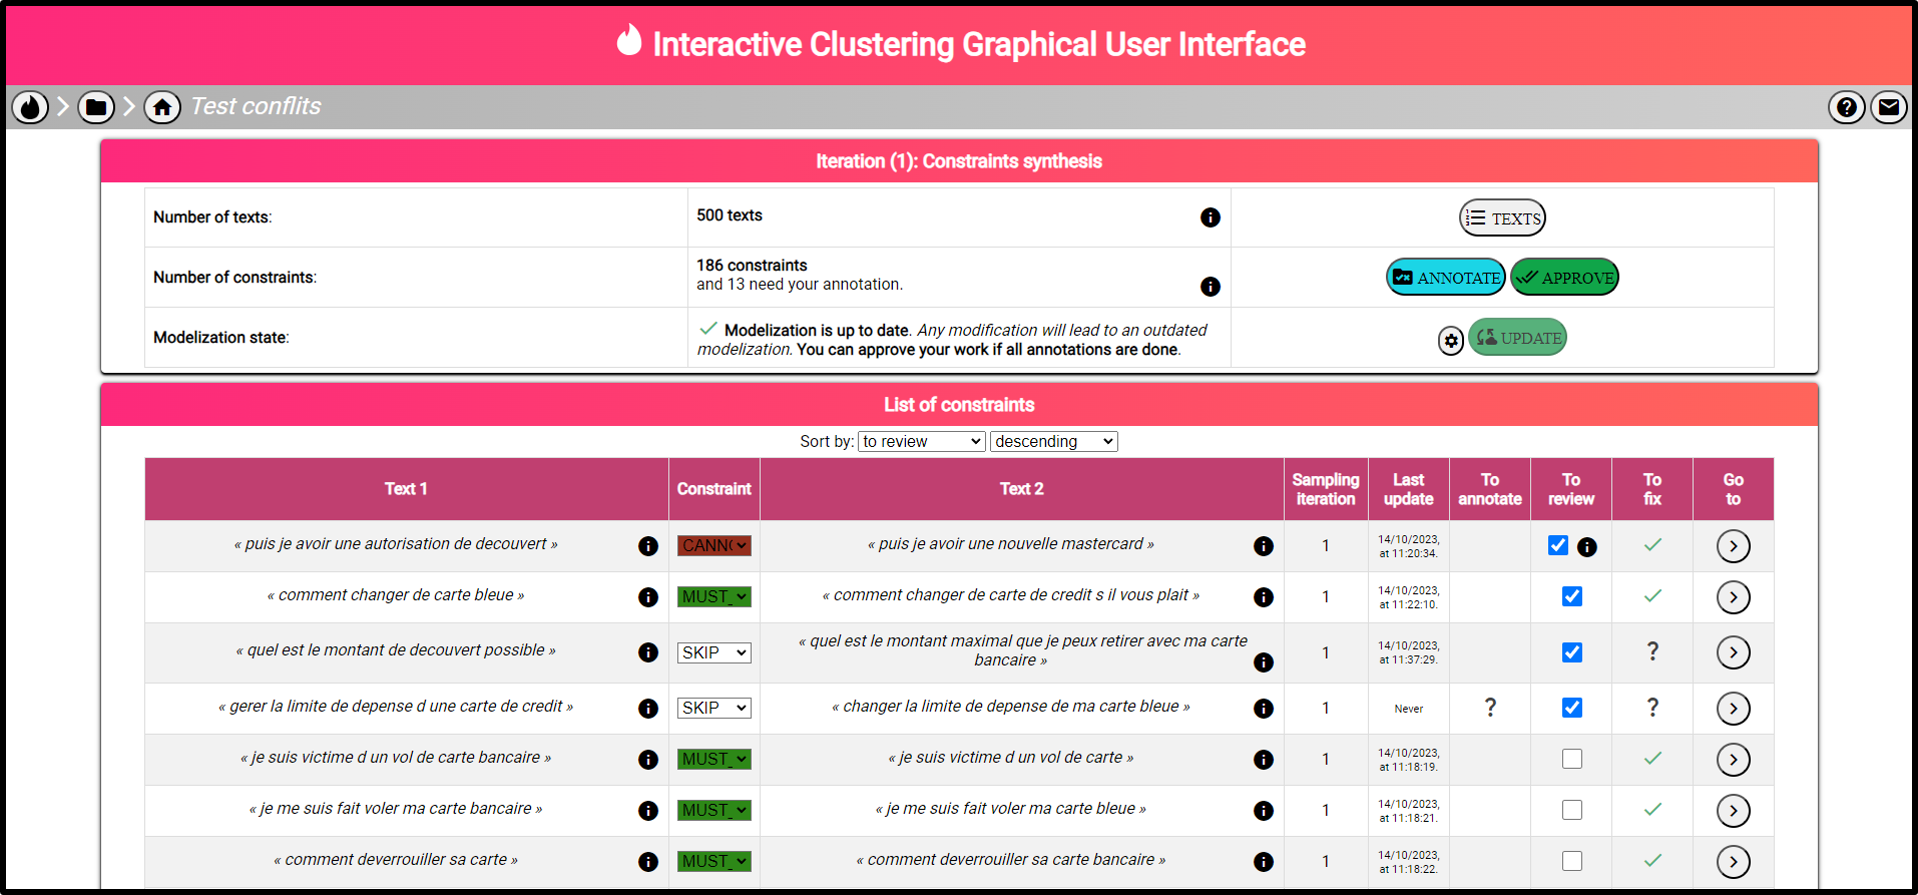
\includegraphics[width=0.95\textwidth]{figures/interactive-clustering-application-contraintes}
				\caption{
					Capture d'écran de l'application web implémentant notre méthodologie de \texttt{Clustering Interactif} : \textbf{page d'inventaire des contraintes}.
				}
				\label{figure:C-WEB-APPLICATION-INVENTAIRE-CONTRAINTES}
			\end{figure}
			
			% Description générale.
			Cette page permet de lister les contraintes du projet à annoter.
			La page est divisée en deux : la partie supérieure donne des informations générales (\textit{nombre de textes, nombre des contraintes à annoter, rappel de la modélisation en cours}), et la partie inférieure liste les contraintes dans un tableau.
			
			% Boutons accessibles: gestion des contraintes.
			Concernant les informations générales (partie supérieure) :
			\begin{itemize}
				\item Le bouton \textguillemets{\texttt{ANNOTATE}} redirige vers la prochaine contrainte à annoter (s'il en reste) ;
				\item Le bouton \textguillemets{\texttt{UPDATE}} permet de mettre à jour la modélisation si des contraintes ont été ajoutées, des paramètres de prétraitements ou de vectorisation ont été mis à jour, ou si des textes ont été modifiés : cette action est exécutée en tâche de fond.
				La couleur de se bouton est définie par le diagramme d'état (cf. \textsc{Figure~\ref{figure:C-WEB-APPLICATION-DIAGRAMME-ETATS}}) ;
				\item Le bouton \textguillemets{\texttt{TEXTS}} mène vers la page d'inventaire et de gestion des données du projet (cf. \textsc{Figure~\ref{figure:C-WEB-APPLICATION-INVENTAIRE-TEXTES}}).
			\end{itemize}
			
			% Boutons accessibles: liste des contraintes.
			Concernant le tableau listant les contraintes (partie inférieure) :
			\begin{itemize}
				\item Les deux textes d'une même contrainte sont affichés de part et d'autre de la valeur annotée : \textcolor{colorApplicationMUSTLINK}{\texttt{MUST-LINK}}, \textcolor{colorApplicationCANNOTLINK}{\texttt{CANNOT-LINK}} ou \texttt{SKIP} (\textit{pour une contrainte non-annotée ou temporairement ignorée}) ;
				\item Il est possible de marquer une contrainte pour la revoir plus tard grâce à la coche \textguillemets{\textcolor{colorApplicationREVIEW}{\faCheckSquare}} ;
				\item Le bouton \textguillemets{\faAngleRight} à droite permet d'accéder à la page d'annotation de cette contrainte (cf. \textsc{Figure~\ref{figure:C-WEB-APPLICATION-ANNOTATION}}) ;
				\item Diverses informations sont disponibles à la droite du tableau : l'itération à laquelle la contrainte a été échantillonnée, sa dernière date de modification, son besoin d'annotation (\textit{\textguillemets{\faQuestion} pour une contrainte encore jamais été annotée}), et la présence ou non de conflits (\textit{\textguillemets{\textcolor{colorApplicationMUSTLINK}{\faCheck}} ou \textguillemets{\textcolor{colorApplicationERROR}{\faExclamation}}}) ;
				\item En haut du tableau, il est possible de trier les contraintes suivant différents critères (\textit{ordre alphabétique, valeur d'annotation, date d'échantillonnage ou de modification, présence de conflit, ...}) ;
				\item \textbf{Attention} : Toute action de modification de la valeur d'annotation nécessite de mettre à jour la modélisation par la suite ;
				De plus, cette action est désactivée si le projet n'est pas à l'étape d'annotation (cf. diagramme d'états en \textsc{Figure~\ref{figure:C-WEB-APPLICATION-DIAGRAMME-ETATS}}) ;
				\item \textit{Note} : Si une contrainte concerne au moins un texte qui a été supprimé (cf. \textsc{Figure~\ref{figure:C-WEB-APPLICATION-INVENTAIRE-TEXTES}}), la contrainte n'apparaît pas dans ce tableau mais existe toujours dans l'application (\textit{elle n'est plus prise en compte}).
			\end{itemize}
	
	
	%%%
	%%% Subsection C.2.4: Annotation et Conflits.
	%%%
	\newpage
	\subsection{Annotation et Conflits}
	\label{annex:C.2.4-DESCRIPTION-IMPLEMENTATION-INTERACTIVE-CLUSTERING-GUI-ANNOTATION}
	
	
		%%% Page d'annotation d'une contrainte
		%\newpage
		\paragraph{Page d'annotation d'une contrainte (\textsc{Figure~\ref{figure:C-WEB-APPLICATION-ANNOTATION}} et \textsc{Figure~\ref{figure:C-WEB-APPLICATION-CONFLIT}}) :}
		
			% Capture d'écran: annotation.
			\begin{figure}[H]
				\centering
				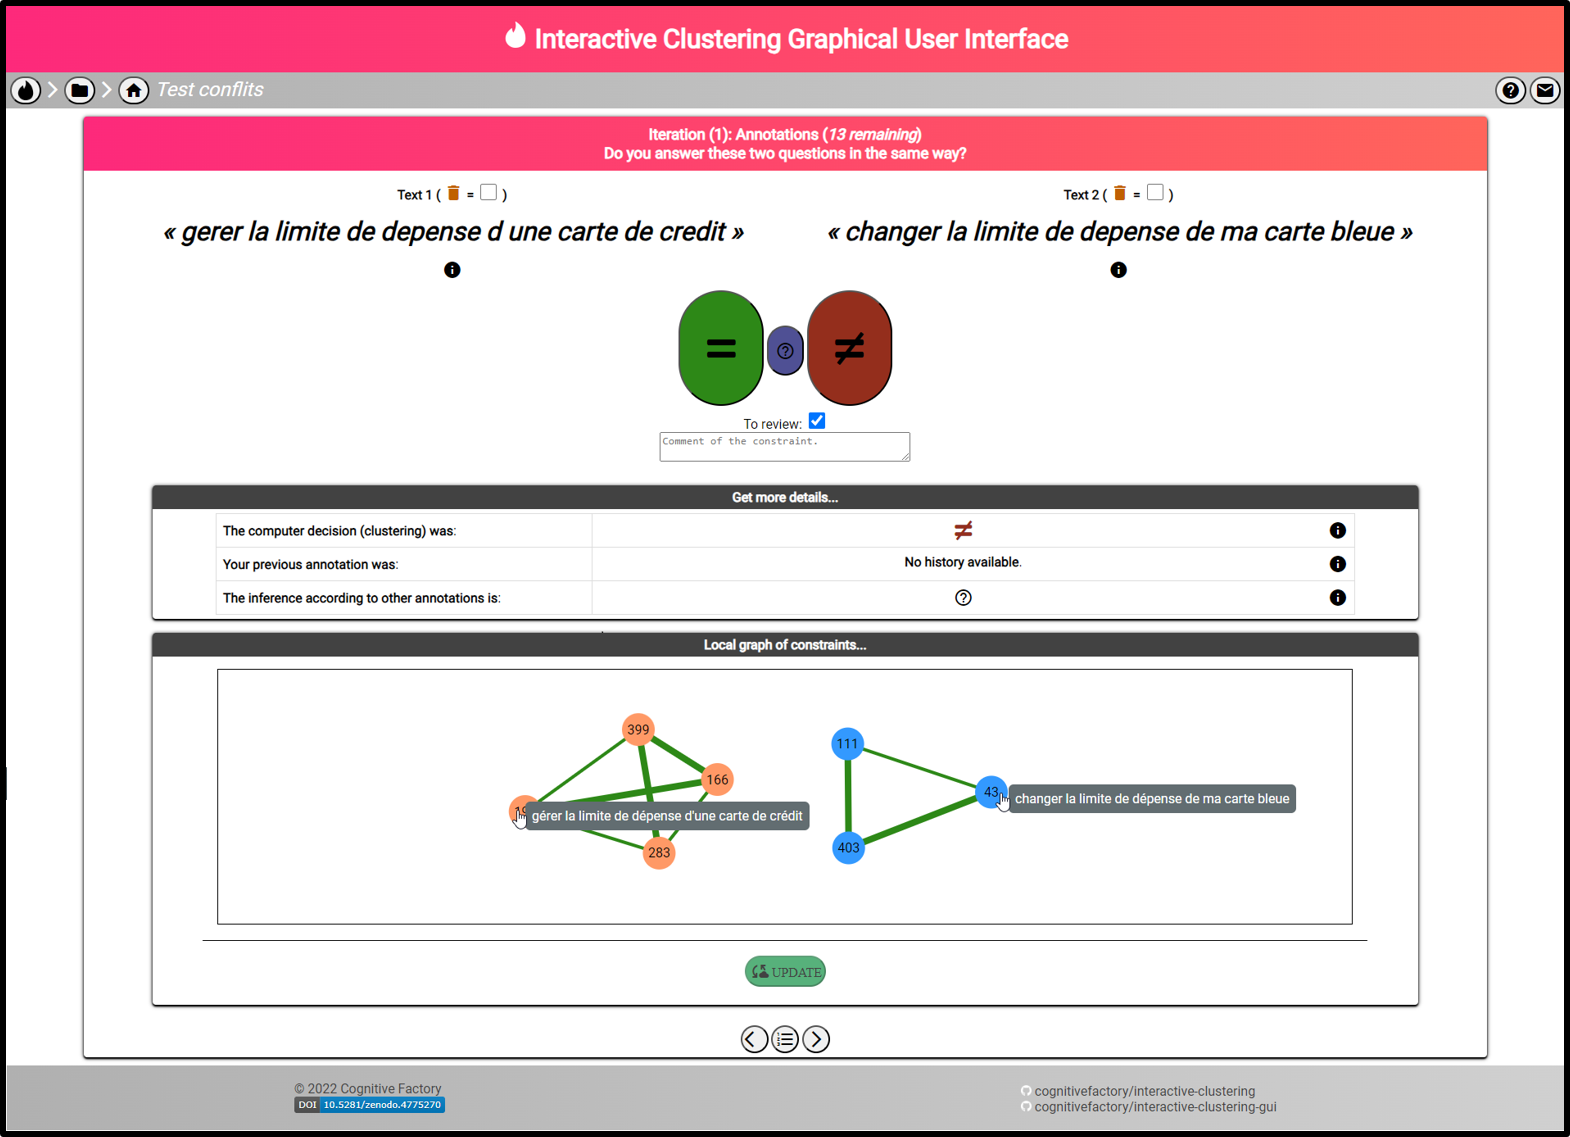
\includegraphics[width=0.95\textwidth]{figures/interactive-clustering-application-annotation-0full}
				\caption{
					Capture d'écran de l'application web implémentant notre méthodologie de \texttt{Clustering Interactif} : \textbf{page d'annotation d'une contrainte}.
				}
				\label{figure:C-WEB-APPLICATION-ANNOTATION}
			\end{figure}
			
			% Description générale.
			Cette page est le coeur de cette application d'annotation : la partie supérieure permet d'annoter une contraintes entre deux textes, les parties inférieures sont des détails (éléments repliés par défaut).
			
			% Boutons accessibles: annotation.
			Concernant l'annotation de la contrainte (partie supérieure) :
			\begin{itemize}
				\item Les deux textes de la contrainte sont affichés en haut du bloc d'annotation ;
				\item Les deux boutons principaux d'annotation sont le \textguillemets{\textcolor{colorApplicationMUSTLINK}{\faEquals}} pour un \texttt{MUST-LINK} et le \textguillemets{\textcolor{colorApplicationCANNOTLINK}{\faNotEqual}} pour un \texttt{CANNOT-LINK}.
				Les raccourcis claviers de ses boutons sont respectivement \textguillemets{\texttt{A}} (\textit{accept}) et \textguillemets{\texttt{R}} (\textit{reject}).
				Il est aussi possible d'ignorer la contrainte avec le bouton \textguillemets{\textcolor{colorApplicationSKIP}{\faQuestion}} (raccourcis avec la barre espace) ;
				\item Si c'est la première fois que cette contrainte est annotée, la prochaine contrainte est automatiquement chargée lors d'un choix d'annotation (\textguillemets{\textcolor{colorApplicationMUSTLINK}{\faEquals}}, \textguillemets{\textcolor{colorApplicationCANNOTLINK}{\faNotEqual}} ou \textguillemets{\textcolor{colorApplicationSKIP}{\faQuestion}}).
				Sinon, une confirmation est demandée pour valider le changement de la valeur de la contrainte ;
				\item Une gestion de revue d'annotation est possible grâce à un champ de commentaire, et \textguillemets{\textcolor{colorApplicationREVIEW}{\faCheckSquare}} permet de marquer la contrainte pour la pour revoir plus tard ;
				\item Grâce à l'icône info-bulle, il est possible d'afficher la version non-prétraitée de chaque texte
				De plus, grâce à la coche \textguillemets{\textcolor{colorApplicationDELETE}{\faTrash}}, il est possible de supprimer (\textit{ne plus prendre en compte}) un texte non pertinent pour le projet : la contrainte sera alors masquée de la liste des contraintes ;
				\item \textbf{Attention} : Toute action de modification de la valeur d'annotation nécessite de mettre à jour la modélisation par la suite.
				De plus, cette action est désactivée si le projet n'est pas à l'étape d'annotation (cf. diagramme d'états en \textsc{Figure~\ref{figure:C-WEB-APPLICATION-DIAGRAMME-ETATS}}) ;
			\end{itemize}
			
			% Boutons accessibles: détails.
			Concernant les détails sur la contraintes (partie inférieure) :
			\begin{itemize}
				\item L'encadré du milieu donne quelques informations sur l'annotation : ce qu'a effectué la machine lors de la précédente étape de \textit{clustering} (même \textit{cluster} ou différentes \textit{cluster} ?), l'historique de ce que l'annotateur a renseigné au préalable, et la déduction faite par le gestionnaire de contraintes grâce aux propriétés de transitivité ;
				\item L'encadré du bas propose une visualisation du graphe de contraintes à l'aide de la librairie \texttt{d3js} \footnote {
					\url{https://d3js.org/}
				} ;
				\item Les boutons en bas de page permettent de naviguer entre les pages d'annotation (boutons \textguillemets{\faAngleLeft} et \textguillemets{\faAngleRight}) ou à revenir vers la page d'inventaire des contraintes (bouton \textguillemets{\faList}, cf. \textsc{Figure~\ref{figure:C-WEB-APPLICATION-INVENTAIRE-CONTRAINTES}}).
			\end{itemize}
			
			% Capture d'écran: conflit d'annotation.
			\begin{figure}[H]
				\centering
				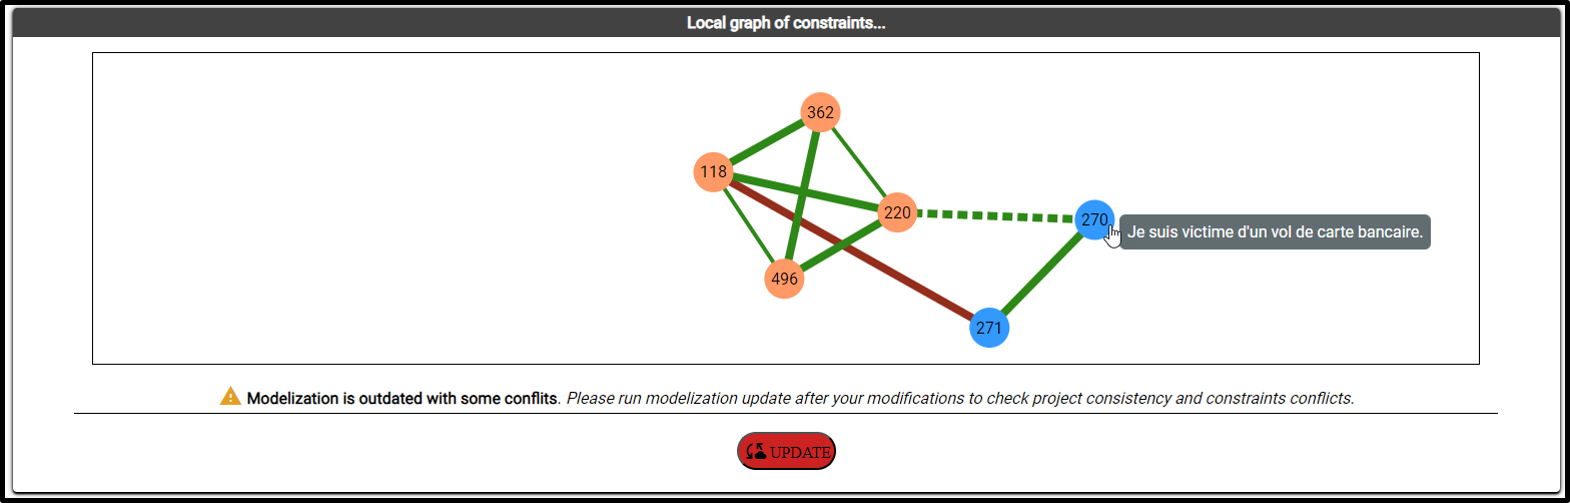
\includegraphics[width=0.95\textwidth]{figures/interactive-clustering-application-annotation-4conflit}
				\caption{
					Capture d'écran de l'application web implémentant notre méthodologie de \texttt{Clustering Interactif} : \textbf{graphe de contraintes présentant un conflit d'annotation}.
				}
				\label{figure:C-WEB-APPLICATION-CONFLIT}
			\end{figure}
			
			% Graphe de contraintes.
			Concernant le graphe local de contraintes :
			\begin{itemize}
				\item Les cercles représentent les données : chaque numéro correspond à un identifiant, et leurs textes respectifs sont visibles par un survol de souris.
				Ces cercles peuvent être déplacés pour une meilleur visibilité ;
				\item Les liens entre les cercles représentent les contraintes : en \textcolor{colorApplicationMUSTLINK}{\textbf{vert}} pour les \texttt{MUST-LINK} et en \textcolor{colorApplicationCANNOTLINK}{\textbf{rouge}} pour les \texttt{CANNOT-LINK}, en \textbf{gras} pour les contraintes annotées et en \textit{fin} pour les contraintes déduites par transitivité, et en \texttt{pointillés} pour les conflits détectés.
				Un clic de souris sur un lien redirige vers la page d'annotation de la contrainte associée (si elle existe) ;
				\item Comme il peut y avoir un nombre important de contraintes dans un projet, ce graphe ne représente que la partie des contraintes impliquées dans l'annotation des deux textes de cette page : nous retrouvons ainsi les deux textes en cours d'annotation et leurs composants connexes respectifs (voir \textsc{Section~\ref{annex:C.1.2-DESCRIPTION-IMPLEMENTATION-INTERACTIVE-CLUSTERING-GESTION-DES-CONTRAINTES}}) ;
				\item Dans l'exemple en \textsc{Figure~\ref{figure:C-WEB-APPLICATION-CONFLIT}}, nous pouvons voir le conflit suivant : \textbf{(1)} $118$ et $270$ doivent être séparés car $118$ est différent de $271$ qui est similaire à $270$, mais \textbf{(2)} $118$ et $270$ doivent être rapprochés car $118$ est similaire à $220$ qui est similaire à $270$...
				\item \textbf{Attention} : En cas de conflit, plusieurs boutons deviennent \textcolor{colorApplicationERROR}{\textbf{rouge}}, et l'approbation de la modélisation est désactivée tant que le conflit n'est pas résolu.
			\end{itemize}